\documentclass[conference]{IEEEtran}
\usepackage[utf8]{inputenc}
\usepackage[spanish]{babel}
\usepackage{graphicx}
\usepackage{float}
\usepackage[hidelinks]{hyperref}
\graphicspath{{assets/}}
\IEEEoverridecommandlockouts
\def\BibTeX{{\rm B\kern-.05em{\sc i\kern-.025em b}\kern-.08em
    T\kern-.1667em\lower.7ex\hbox{E}\kern-.125emX}}

\begin{document}
\title{Grupo 1: Estación de confort para puesto de estudio}

\author{
    \IEEEauthorblockN{1\textsuperscript{st} Kevin Ramírez Corrales}
    \IEEEauthorblockA{\textit{Universidad Cooperativa de Colombia}\\
    kevin.ramirezcorr@campusucc.edu.co}
    \and
    \IEEEauthorblockN{2\textsuperscript{nd} Mauro Jaramillo Zapata}
    \IEEEauthorblockA{\textit{Universidad Cooperativa de Colombia}\\
    mauro.jaramillo@campusucc.edu.co}
    \and
    \IEEEauthorblockN{3\textsuperscript{rd} Jaime Andrés Anchico}
    \IEEEauthorblockA{\textit{Universidad Cooperativa de Colombia}\\
    officialmarker88@gmail.com}
    \and
    \IEEEauthorblockN{4\textsuperscript{th} José Manuel Padilla}
    \IEEEauthorblockA{\textit{Universidad Cooperativa de Colombia}\\
    jose.padillacal@campusucc.edu.co}
}

\maketitle

\begin{abstract}
En este proyecto se desarrolló una estación de confort orientada a mejorar las condiciones 
ambientales de un puesto de estudio. El sistema mide temperatura e iluminación, mostrando 
los datos en una pantalla LCD I2C y tomando decisiones automáticas como la activación de 
ventilación y el ajuste de iluminación mediante PWM. Además, se implementaron modos de 
operación manual y automático, junto con técnicas como antirrebote y temporización con millis(), 
permitiendo un funcionamiento estable y continuo.
\end{abstract}

\begin{IEEEkeywords}
Arduino, sensores, automatización, PWM, LCD I2C, millis()
\end{IEEEkeywords}

\section{Introducción}
Las condiciones ambientales influyen directamente en el rendimiento académico y laboral. 
Factores como la temperatura y la iluminación pueden afectar la concentración, la comodidad 
y la productividad. Por esta razón, se propone el desarrollo de un sistema automatizado capaz 
de supervisar estas variables y actuar de manera inteligente para mejorar el entorno de estudio.

\section{Objetivos}
\subsection{Objetivo General}
Diseñar una estación de confort que supervise y mejore las condiciones de temperatura e iluminación
en un puesto de estudio.
\subsection{Objetivos Específicos}
\begin{itemize}
    \item Medir la temperatura ambiente utilizando un sensor DS18B20.
    \item Detectar el nivel de iluminación usando una LDR.
    \item Visualizar la información en una pantalla LCD I2C.
    \item Implementar modos de operación manual y automático.
    \item Controlar ventilación mediante un motor DC.
    \item Regular la iluminación utilizando PWM.
\end{itemize}

\section{Metodología}
El desarrollo del proyecto se realizó de manera colaborativa, distribuyendo tareas entre 
programación, montaje y documentación.

Inicialmente se diseñó el circuito en protoboard, integrando sensores, actuadores y la pantalla LCD. 
Posteriormente, se desarrolló el código en Arduino IDE, implementando la lectura de sensores, 
control de actuadores y visualización de datos.

Se utilizó la función millis() para evitar bloqueos en la ejecución del programa, permitiendo 
una respuesta más fluida del sistema.

\section{Diseño del Sistema}
\subsection{Diagrama de Funcionamiento}
El sistema funciona a partir de la lectura constante de los sensores. Dependiendo de los valores
obtenidos, el sistema toma decisiones automáticamente o permite control manual.
\subsection{Condiciones de Operación}

\begin{table}[h]
    \centering
    \begin{tabular}{|c|c|c|}
        \hline
            Condición & Acción & Modo \\
        \hline
            Temp $>$ 28°C & Activar ventilación & Automático \\
        \hline
            Temp $\leq$ 28°C & Desactivar ventilación & Automático \\
        \hline
            Luz baja $<$ 300 & Aumentar iluminación & Automático \\
        \hline
            Luz alta $\geq$ 300 & Disminuir iluminación & Automático \\
        \hline
            Botón Manual & Cambiar modo & Manual \\
        \hline
    \end{tabular}
    \caption{Condiciones de operación del sistema}
\end{table}

\section{Simulación del sistema}

\begin{figure}[H]
    \centering
    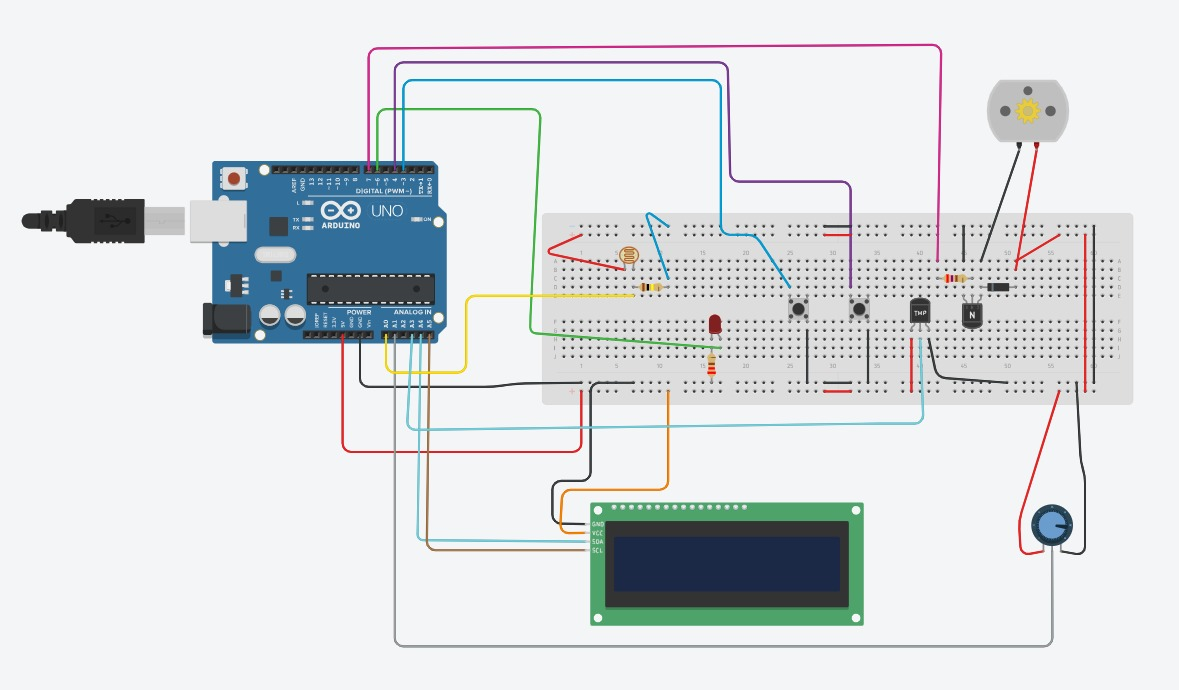
\includegraphics[width=0.9\linewidth]{simulacion.jpeg}
    \caption{Simulación del sistema en TinkerCAD}
\end{figure}

En la simulación se validó el funcionamiento general del sistema, adaptando algunos componentes 
debido a las limitaciones del entorno virtual.

\section{Montaje Físico}

\begin{figure}[H]
    \centering
    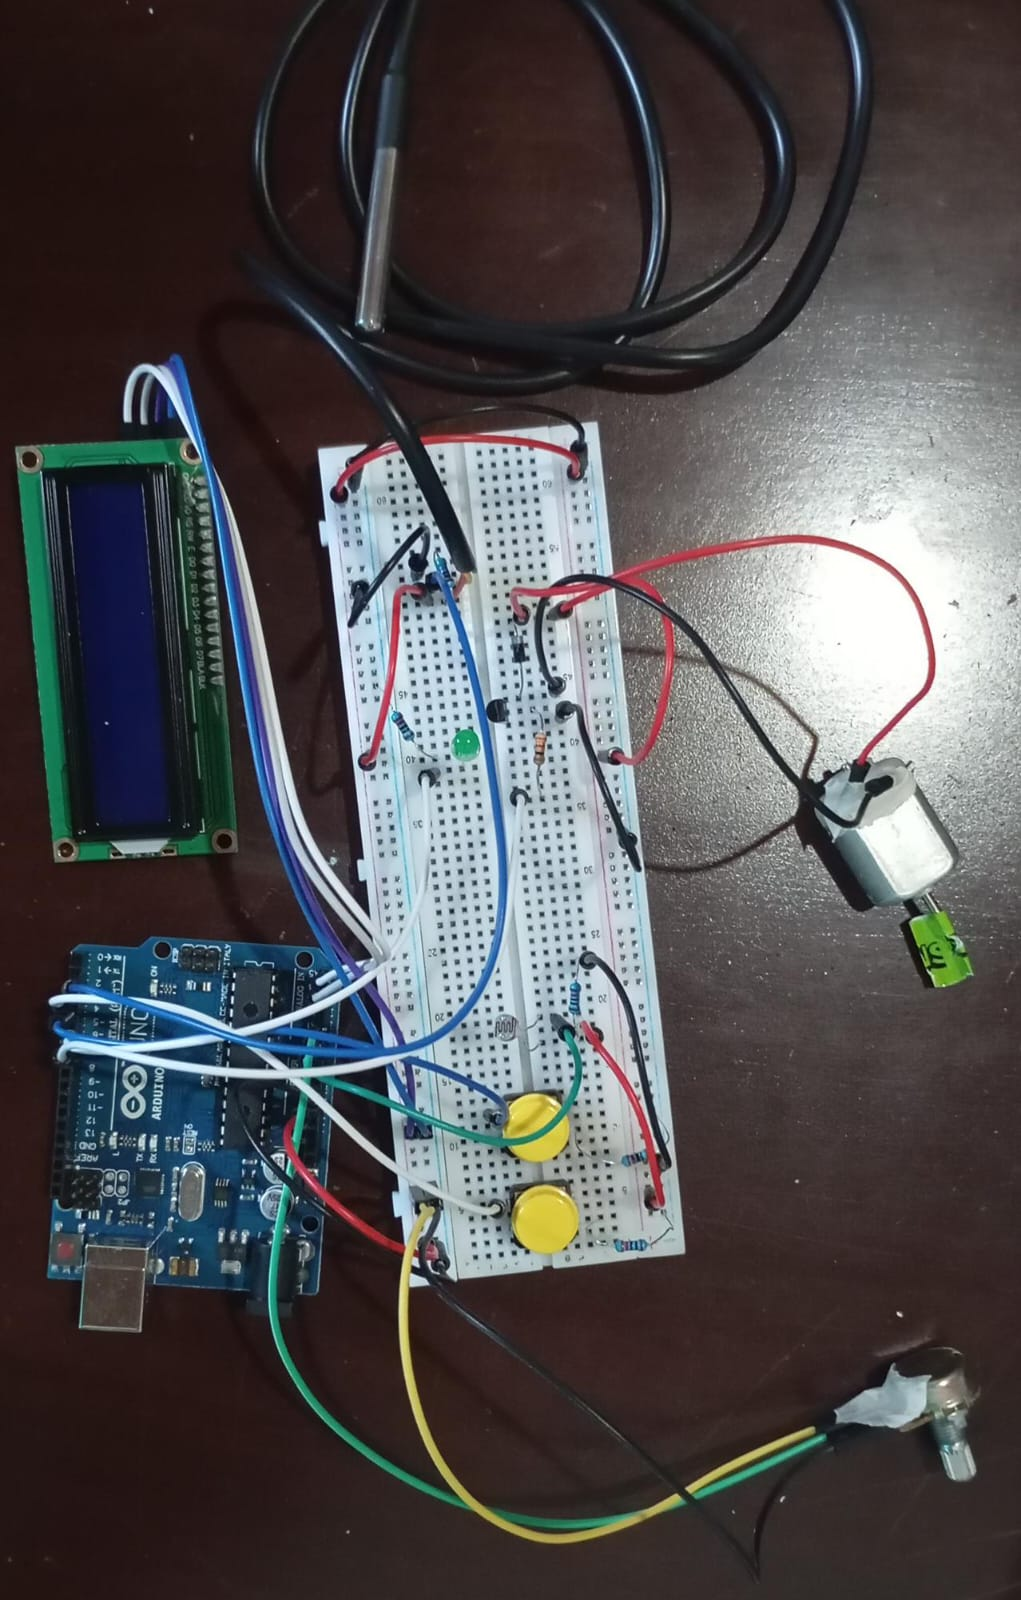
\includegraphics[width=0.9\linewidth]{fisico.jpeg}
    \caption{Montaje físico del sistema}
\end{figure}

El montaje físico permitió comprobar el comportamiento real del sistema, asegurando la correcta 
integración entre sensores, actuadores y visualización.

\section{Desarrollo}

\subsection{Lectura de sensores}
El sensor DS18B20 se utilizó para medir la temperatura con buena precisión. Este sensor trabaja
de forma digital, lo que facilita su lectura. Por otro lado la LDR entrega valores analógicos
que dependen de la cantidad de luz recibida.

\subsection{Visualización en el LCD}
Se utilizó una pantalla LCD con comunicación I2C para mostrar:
\begin{itemize}
    \item Temperatura actual en °C.
    \item Nivel de iluminación.
    \item Modo de operación (Automático o Manual).
\end{itemize}
Esto permite al usuario entender fácilmente el estado del sistema.

\section{Decisiones técnicas}
\begin{itemize}
\item En el simulador TinkerCAD se utilizó el sensor TMP36 en lugar del DS18B20, debido a la 
falta de soporte para las librerías OneWire y DallasTemperature. Esto implicó el uso de un pin 
analógico, ya que el TMP36 trabaja con señales analógicas en lugar de comunicación digital.
\item Para el control del motor DC se empleó un transistor junto con un diodo de protección. 
Esto evita que el Arduino maneje directamente la corriente del motor, reduciendo el riesgo de daño 
en la placa y protegiendo contra picos de voltaje.
\item Se evitó el uso de la función lcd.clear(), ya que genera parpadeos en la pantalla. 
En su lugar, se implementó la sobreescritura de caracteres, mejorando la experiencia del usuario.
\item Se utilizó millis() en lugar de delay() para lograr una ejecución no bloqueante, permitiendo 
la lectura continua de sensores y una mejor respuesta del sistema.
\item Los botones fueron configurados como INPUT\_PULLUP para simplificar el circuito y eliminar 
la necesidad de resistencias externas.
\item Se implementó una validación lógica en el control del motor, evitando que el usuario pueda 
modificar su estado en modo automático, garantizando coherencia en el funcionamiento del sistema.
\item Se empleó una resistencia de 220 ohmios para proteger el LED y una resistencia de 4.7k ohmios 
para asegurar lecturas estables en el sensor.
\item Se seleccionó una pantalla LCD con interfaz I2C para reducir la cantidad de conexiones y 
optimizar el espacio en el montaje.
\end{itemize}

\section{Conclusión}
El desarrollo de este proyecto permitió integrar diferentes conceptos de electrónica y programación, 
logrando un sistema funcional capaz de mejorar las condiciones de un entorno de estudio. 
Además, se evidenció la importancia de la toma de decisiones técnicas para garantizar la estabilidad, 
seguridad y eficiencia del sistema.

\section{Recursos del Proyecto}

A continuación, se presentan los enlaces asociados al desarrollo del proyecto, incluyendo 
el código fuente, la simulación y el video demostrativo.

\subsection{Código fuente}
El código del proyecto, incluyendo los sketches utilizados y el desarrollo del informe en LaTeX, 
se encuentra disponible en el siguiente repositorio:

\begin{itemize}
    \item \textbf{Repositorio (carpeta del proyecto):} \\
    \url{https://github.com/KevinRCorrales/tex_informes/tree/main/automatas%2Fmomento2}
\end{itemize}

\subsection{Simulación}
La simulación del sistema fue desarrollada en TinkerCAD y puede visualizarse en el siguiente enlace:

\begin{itemize}
    \item \textbf{Simulación en TinkerCAD:} \\
    \url{https://www.tinkercad.com/things/gPFZ0BTAJCn/editel?returnTo=%2Fthings%2FflHpOFbJ1CN-arduino-simulator-and&sharecode=WvfsPZ4p9TMGW3o0mcmmQWlGb7kjKji6UtBTkyA_ty0}
\end{itemize}

\subsection{Video demostrativo}
Se realizó un video donde se evidencia el funcionamiento del sistema, tanto en simulación como en montaje físico:

\begin{itemize}
    \item \textbf{Video del proyecto:} \\
    \url{https://youtu.be/TtyDQYm5Pbo?si=Wntlrex-VdIHelA6}
\end{itemize}
\end{document}
